%!TEX root=main.tex
\section{Implementation}
\label{clicknp:sec:impl}

\subsection{\name\ tool-chain and hardware setup}
We have built a \name\ compiler which serves as the front-end of the \name\ tool-chain (\S\ref{clicknp:subsec:toolchain}).  
%
For the host program, we use Visual C++ as the backend. We further integrate Altera OpenCL SDK (v15.1)~\cite{aoc} and 
Xilinx Vivado HLS (v2015.4)~\cite{vivado} as the backend for the FPGA program.
%
The \name\ compiler contains 4,925 lines of C++ code, which parses configuration file and element declarations, 
performs optimizations in \S\ref{clicknp:sec:optimization}, and generates code specific for each commercial HLS tool.
% Cross platform.
When working with Altera OpenCL, each \name\ element is compiled into a \textit{kernel} and 
the connections between elements are translated into Altera extended channels.
When using Xilinx Vivado HLS, we compile each element into an IP core and 
use AXI streams to implement connections between elements.
%
An element can also be compiled to CPU binary and the manager thread will create one worker thread for each host element.
%
Each connection between a host and a FPGA element is mapped to a \textit{slot} of the PCIe I/O 
channel (\S\ref{clicknp:subsec:pcie}).

Our hardware platform is based on Altera Stratix V FPGA with the Catapult shell~\cite{putnam2014reconfigurable}.
The Catapult shell also contains an OpenCL specific runtime, so that the \name\ role can communicate with the shell 
through this runtime layer.
The FPGA board has a PCIe Gen2 x8 interface, 4GB onboard DDR memory and two 40G Ethernet ports. 
%
By the time of writing this paper, we do not get a Xilinx hardware platform. 
Therefore, the primary system evaluations are based on the Altera platform using \name+OpenCL, 
and we use the reports generated by Vivado HLS, \eg, frequency and area cost, to understand 
the performance of \name+Vivado.

\subsection{\name\ element library}
\label{clicknp:subsec:lib}

\begin{table*}[t!]
	\centering
	\caption{A selected set of key elements in \name. }
	\label{clicknp:tab:elements}
	\scalebox{0.9}{
		\begin{tabular}{l|l|l|p{1cm}|p{2.2cm}|p{2cm}|p{1.3cm}|r|r}
			\toprule
			&	&	& \multicolumn{4}{c|}{Performance} & \multicolumn{2}{c}{Resource (\%)} 			\\
			\cline{4-7} \cline{8-9}  

 Element 	& Configuration & Optimizations & Fmax (MHz) & Peak \quad \quad Throughput & Speedup\quad (FPGA/CPU) & Delay (cycles) & LE & BRAM \\
			\midrule
			L4\_Parser (A1-5)  & N/A & REG & 221.93 & 113.6 Gbps & 31.2x / 41.8x & 11 & 0.8\% & 0.2\% \\
			IPChecksum (A1-4) & N/A & UL & 226.8 & 116.1 Gbps & 33.1x / 55.1x & 18 & 2.3\% & 1.3\% \\
			NVGRE\_Encap (A1,4) & N/A & REG, UL & 221.8 & 113.6 Gbps & 35.5x / 42.9x & 9 & 1.5\% & 0.6\% \\
			\midrule
			AES\_CTR (A3) & 16B block & UL & 217.0 & 27.8 Gbps & 79.9x / 255x & 70 & 4.0\% & 23.1\% \\
			SHA1 (A3) & 64B block & MS, UL & 220.8 & 113.0 Gbps & 157.5x / 83.1x & 105 & 7.9\% & 6.6\% \\
			\midrule
			\midrule
			CuckooHash (A2) & 128K entries & MS, UL, DW & 209.7 & 209.7 Mpps & 43.6x / 57.5x & 38 & 2.0\% & 65.5\% \\
			HashTCAM (A2) & 16 x 1K & MS, UL, DW & 207.4 & 207.4 Mpps & 155.9x / 696x & 48 & 18.7\% & 22.0\% \\
			LPM\_Tree (A2) & 16K entries & MS, UL, DW & 221.8 & 221.8 Mpps & 34.5x / 45.2x & 181 & 4.3\% & 13.2\% \\
			FlowCache (A4) & 4-way, 16K & MS, DW & 105.6 & 105.6 Mpps & 55.8x / 21.5x & 27 & 5.6\% & 46.9\% \\
			\midrule

			SRPrioQueue (A5) & 32 Pkts buffer & REG, UL & 214.5 & 214.5 Mpps & 150.3x / 28.6x & 41 & 2.6\% & 0.6\% \\
			RateLimiter (A1,5) & 16K flows & MS, DW & 141.5 & 141.5 Mpps & 7.0x / 65.3x & 14 & 16.9\% & 14.1\% \\
\bottomrule

	\multicolumn{9}{l} {\textbf{Optimization method.} REG=Using Registers; MS=Memory Scattering; UL=Unroll Loop; DW=Delay Write.} \\
	\multicolumn{9}{l} {\parbox{\textwidth}{The \textbf{Speedup} column compares the performance between
	the optimized version and our earlier implementation without applying techniques discussed in \S\ref{clicknp:sec:optimization} as well as a CPU implementation.}}

		\end{tabular} 

	}
\end{table*}

We have implemented a \name\ element library that contains nearly 100 elements. 
Part of them (20\%) are derived directly from the Click Modular Router, 
but re-factored using the \name\ framework. 
These elements cover a large range of basic operations of NFs, 
including packet parsing, checksum computing,
encap/decap, hash tables, longest prefix matching (LPM), 
rate limiting, cryptographic, and packet scheduling. 
%
Due to the modular architecture of \name, the code size of each element is modest. 
The mean line-of-code (LoC) of an element is 80 and 
the most complex element, \textit{PacketBuffer}, has 196 lines of C code. 
% 
Table~\ref{clicknp:tab:elements} presents a selected set of key elements we have implemented in \name. 
Beside element names, we also mark the demonstration NFs (A1\approx A5, discussed in \S\ref{clicknp:sec:application}) in 
which the element is used.
%
We have heavily applied the optimization techniques discussed earlier in \S\ref{clicknp:subsec:paral_in_elem} to 
minimize memory dependency and balance pipeline stages.
We summarize the optimization techniques used for each element in the 3rd column.
For the top part of Table~\ref{clicknp:tab:elements}, the element needs to touch every byte of a packet. We show the throughput in Gbps.
The elements in the bottom part of the table, however, process only the packet header (metadata). Therefore, it makes more
sense to measure the throughput using packet per second.
%
We note that the throughput measured in Table \ref{clicknp:tab:elements} is the maximal throughput that the corresponding element can achieve.
When they work in a real NF, other components, \eg the Ethernet port, may be the bottleneck.
%
As a reference, we compare the optimized version to our earlier  
implementation on FPGA without applying the techniques discussed in \S\ref{clicknp:sec:optimization} as well as a CPU implementation.
Clearly, after optimization, all these elements can process packet very efficiently, achieving 7\approx 157x speedup compared to our naive FPGA implementation, and 21\approx 696x speedup over a software implementation on one CPU core.
This performance gain comes from the ability to utilize the vast parallelism in FPGA.
%
Considering the power footprint of FPGA (\approx 30W) and CPU (\approx 5W per core), 
\name\ elements are 4\approx 120x more power efficient than CPU. 

We also show the processing latency of each element in Table~\ref{clicknp:tab:elements}. 
As we see, this latency is low: The mean is $0.19 \mu s$ and the maximum is merely $0.8 \mu s$ (LPM\_Tree).
% cost
The last two columns summarize the resource utilization of each element. The utilization is normalized to
the capacity of the FPGA chip. 
We can see most elements use only a small number of logic elements.
This is reasonable as most operations on packets are simple. 
HashTCAM and RateLimiter have moderate usage of LEs because these elements have larger arbitration logic. 
%
The BRAM usage, however, heavily relies on configurations of elements. For example, the BRAM usage grows linearly 
with the number of entries supported in a flow table. 
Overall, our FPGA chip has sufficient capacity to support a meaningful 
NF containing a handful elements (\S\ref{clicknp:sec:application}).



\subsection{PCIE I/O channel}
\label{clicknp:subsec:pcie}

As aforementioned, one key property of \name\ is to support joint CPU/FPGA processing. 
We enable this by designing a high-throughput, low latency PCIe I/O channel. 
%
We extend the OpenCL runtime and add a new I/O channel, which is connected to 
a PCIe switch in the shell. 
The PCIe switch will arbitrate the access between the newly added I/O channel
and other components in the shell, \eg, DDR memory controller.

We leverage the PCIe slot DMA engine in Catapult shell \cite{putnam2014reconfigurable}, which divides a PCIe Gen2 x8 link into 64 logical sub-channels, \ie, \textit{slots}.
Each slot has a pair of send and receive buffers for DMA operations.
%
Among 64 slots, 33 are reserved by Shell and the runtime library to control kernels and access on-board DDR, one slot is used for passing signals to \name\ elements. 
The remaining 30 slots, however, are used for data communications among FPGA and CPU elements.
%
To amortize DMA overhead, we aggressively use \textit{batching}. The maximum message size 
is limited at 64KB. 
%The PCIe channel can work in both interrupt or polling mode.



% cmdhub
In FPGA, a special element, called \textit{CmdHub}, which is generated automatically by the \name\ compiler, 
redirects the data from different slots to corresponding FPGA elements 
using FIFO buffers.
% signal slot
\textit{CmdHub} is also used to distribute control signals from the manager 
thread to FPGA elements.
To identify the target element, an element ID is embedded in the signal message,
and \textit{CmdHub} can read the ID and forward the signal message to 
the corresponding element, again through FIFO buffers. 

Figure~\ref{clicknp:fig:pcie} shows a benchmark of our PCIe I/O channel with different number of slots and batch sizes.
As a base-line, we also measure the performance of OpenCL global memory operations -- so far, the only means provided
for CPU/FPGA communication in OpenCL~\cite{opencl}. 
%
We can see that the maximum throughput of a single slot is around 8.4~Gbps. 
With 4 slots, the aggregate throughput of the PCIe I/O channel can reach up to 25.6~Gbps. 
This is the maximum throughput we can get out of our current FPGA chip due to limitation of the clock frequency of the DMA engine. 
However, the throughput of OpenCL is surprisingly low, less than 1~Gbps. This is because the global memory API is designed
to transfer huge amount of data (multiple GB). This may be suitable for applications with large data set, but not for 
network functions that require strong stream processing capability.
Similarly, Figure~\ref{clicknp:fig:pcie}(b) shows the communication latency. Since OpenCL is not optimized for stream processing,
the OpenCL latency is as high as 1~ms, usually unacceptable for network functions. 
In contrast, the PCIe I/O channel has very low latency of 1~$\mu$s in polling mode (one core repeatedly polls status register) and 9~$\mu$s in interrupt mode (with almost zero CPU overhead).

\begin{figure}[t!]
	\centering
	\subfloat[]{
		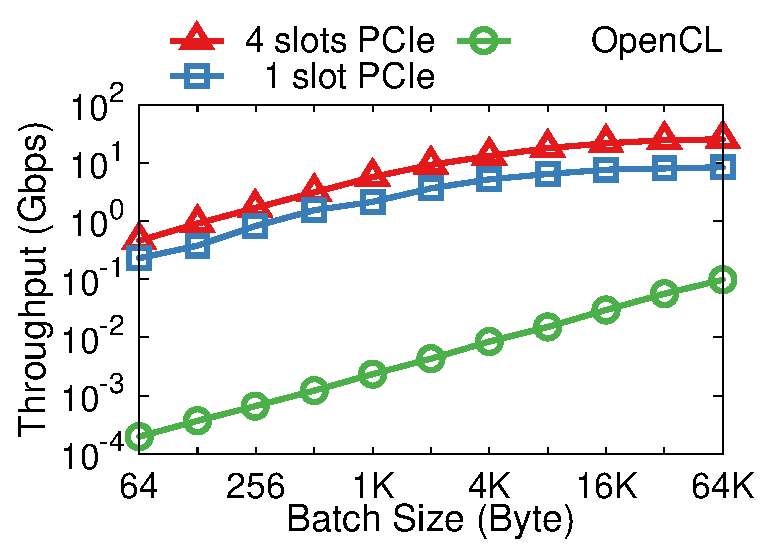
\includegraphics[width=0.5\textwidth]{eval/pcie_1}
	}
	\subfloat[]{
		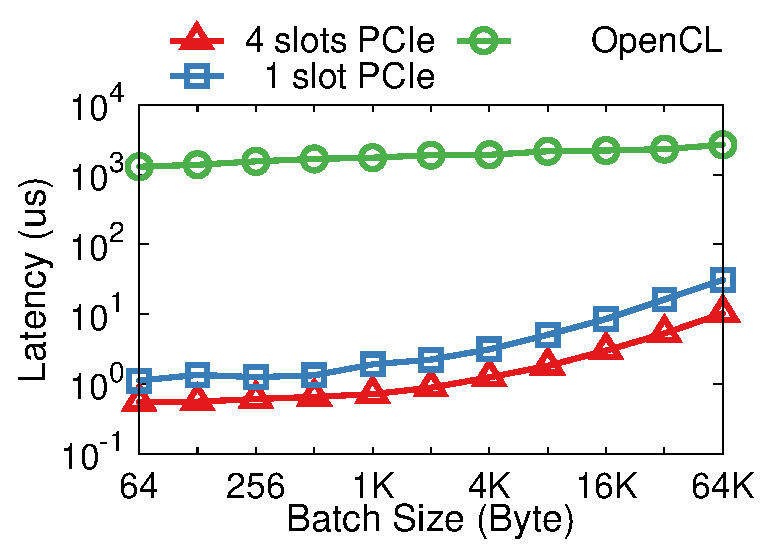
\includegraphics[width=0.5\textwidth]{eval/pcie_2}
	}

	\caption{The performance of the PCIe I/O channel. The y-axis is in logarithmic scale. }

	\label{clicknp:fig:pcie}
\end{figure}

\egg{

\egg{
Control signals can only be generated by the manager thread. 
When the manager thread sends a signal to a target element in FPGA, it will embed the ID of the element in the signal message, and 
passes the message to \textit{CmdHub} through slot 32.
\textit{CmdHub} will parse the message and forward the signal request to corresponding elements, again through FIFO buffers. 
}



\egg{
As aforementioned, OpenCL advocates batch processing model where communication between host program and a kernel in FPGA must go through shared DRAM, and the host program cannot control the kernel while it is running.
We could use a special kernel to proxy messages between host program and the kernel via DRAM, but it incurs \approx1ms latency.
DDR access is performed via PCIe link and raw PCIe latency is merely \approx1$\mu$s. As we improve kernel communication efficiency with channels in place of shared memory, we design a host-kernel communication mechanism with channel abstraction for low latency and high throughput.
We leverage I/O channel in Altera OpenCL and AXI stream in Vivado HLS to connect the Catapult shell to kernels and built a PCIe bypass switch to arbitrate accesses for on-board DRAM and kernel I/O channel.

A PCIe link is split into multiple logically independent \textit{slots} which can operate in parallel.
One slot is reserved for signals. Remaining slots are assigned to channels between host and FPGA elements, so each channel can transfer data in parallel without head-of-line blocking.
On CPU side, each host element is run on a separate core and receives input flits via PCIe by polling or interrupt.
On FPGA side, each element that communicates with host is connected to an inbound demultiplexer and an outbound multiplexer, where load-adaptive batching is performed to improve peak throughput while preserving low latency under light load.
}

\egg{
With polling model, the latency of the PCIe I/O channel  is $< 2 \mu s$ when message size is small, but the latency will reach to $32 \mu s$
for full batched messages.
The interrupt model, however, will increase the latency.
}

\egg{
, where each slot is assigned to one CPU core. Our PCIe channel has two bottlenecks: (1) PCIe Gen2 x8 interface has 32 Gbps bandwidth, (2) PCIe data width is 128b and the clock frequency of Catapult shell is 200 MHz, which limits PCIe throughput to 25.6 Gbps. PCIe I/O channel offers 1\approx2$\mu$s RTT which translates to 400\approx800K host-kernel transactions per second. Polling mode yields lower latency and higher throughput, while interrupt mode latency can be improved by utilizing more cores and PCIe slots. Four CPU cores are sufficient to saturate maximum throughput for both polling and interrupt mode under 64KB batch size. Effectiveness of batching will be further evaluated in traffic dumper application.
}

}
